%% ma: L12-B01-0047
%% lop: 12
%% chuong: 1
%% bai: 1
%% dang: 12.1.21
%% loai: TN4
%% muc: TH
%% dap_an: "C"
%% nguon: "Ảnh giáo viên gửi 05/11/2026 (M11): Kiểm tra giữa HK1 Toán 12 (2026-2027), THPT Hồ Thị Bi (TP.HCM), mã đề 1133, Phần I Câu 23"
%% kien_thuc: "Bài 1 (tính đơn điệu: đọc từ bảng xét dấu đạo hàm)"
%% trang_thai: chinh-thuc
%% ghi_chu: "Đề gốc không kèm đáp án; đã giải độc lập."
\begin{ex}
Cho hàm số $y=f(x)$ xác định trên $\mathbb R$ và có bảng xét dấu đạo hàm như sau:
\begin{center}
\begin{tikzpicture}
  \tkzTabInit[lgt=1.5,espcl=2]{$x$/.8,$f'(x)$/.8}{$-\infty$,$-3$,$0$,$3$,$+\infty$}
  \tkzTabLine{,+,0,-,d,-,0,+,}
\end{tikzpicture}
\end{center}
Mệnh đề nào dưới đây đúng?
\choice{Hàm số $f(x)$ đồng biến trên khoảng $(-3;0)$}{Hàm số $f(x)$ nghịch biến trên khoảng $(-\infty;-3)$}{\True Hàm số $f(x)$ nghịch biến trên khoảng $(0;3)$}{Hàm số $f(x)$ đồng biến trên khoảng $(-\infty;0)$}
\loigiai{Từ bảng xét dấu: $f'(x)>0$ trên $(-\infty;-3)$ và $(3;+\infty)$; $f'(x)<0$ trên $(-3;0)$ và $(0;3)$.
Do đó hàm số đồng biến trên $(-\infty;-3)$, $(3;+\infty)$ và nghịch biến trên $(-3;0)$, $(0;3)$.
Vậy chỉ có mệnh đề C đúng.}
\end{ex}
